\subsection{Allgemein}            
Der Name Edubot bezeichnet sowohl das Softwaresystem als ganzes, als auch den aus Holz gefertigten Roboterarm. Der Roboterarm wird um Missverständnisse zu vermeiden allgemein als "'Edubot Modell"' bezeichnet. Es handelt sich bei diesem Roboterarm um eine Konstruktion mit zwei rotatorischen Achsen die so konzipiert wurde dass eine Erweiterung um diverse Werkzeuge oder weitere Achsen ohne Probleme und mit Hilfe des Handbuchs möglich ist. 

\begin{figure}[H]
  \centering
  \begin{minipage}[t]{12 cm}
  	\centering
  	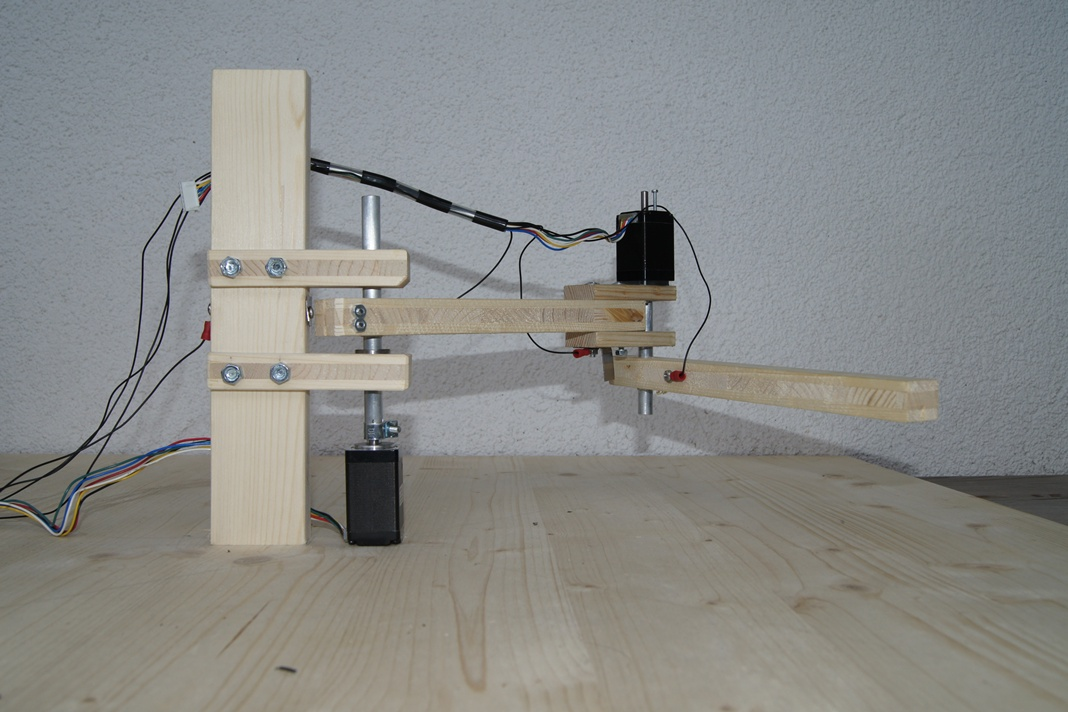
\includegraphics[width=12cm]{images/edubot_photo} 
    \caption{Das Edubot Modell}
  \end{minipage}
\end{figure}

\subsubsection{Aufgaben}
Das Edubot Modell soll als Anschauungsmaterial sowohl für den Unterricht, als für Anlässe wie den Tag der offenen Tür oder sonstige Präsentationszwecke dienen. Der Aufbau des Modells und die verwendete Elektronik wurde bewusst so simpel wie möglich gehalten um es Schülern zu ermöglichen schnell einen Überblick über die Funktionsweise und konstruktionstechnischen Eigenheiten zu erlangen.

\subsubsection{Funktionen}
Das Edubot Vorführmodell verfügt über zwei rotatorische Achsen die auf horizontaler Ebene bewegt werden können. 
Der Roboter besitzt damit zwei Freiheitsgrade und kann auf einer Ebene alle Punkte in einem Nieren-förmigen Arbeitsbereich anfahren. Abhängig vom montierten Werkzeug kann der Roboter beispielsweise dafür verwendet werden einfache Zeichnungen anzufertigen. Ein entsprechendes Werkzeug wird jedoch nicht mitgeliefert und muss selbst konstruiert werden.

\subsubsection{Bedienung}
Als Steuerungsteil des Roboterarms dient ein Mikrocontroller (GHI Embedded Master) welcher sowohl über eine Netzwerkschnittstelle, als auch über einen USB Anschluss verfügt. Zur Übergabe von Befehlen an den Roboter wird ausschließlich die Netzwerkschnittstelle verwendet. Der USB Anschluss  wird nur benötigt um Softwareänderungen am Controller durchzuführen.
Um dem Roboterarm Befehle zu übergeben, muss der Mikrocontroller mithilfe eines normalen Netzwerkkabels mit RJ-45 Steckern an einen Computer angeschlossen werden auf welchem eine Applikation läuft welche auf der mitgelieferten API aufbaut.